\chapter{Implementación}\label{cap:implementacion}

	En este capítulo se va a detallar la implementación, tanto a nivel hardware como software, del sistema de actuación y de cada uno de los bloques que lo componen.

	 El sistema de actuación se ha implementado en una Raspberry PI 2 model B, ya que dispone de un buen procesador, un puerto ethernet para conexión a internet, una buena memoria y varios puertos GPIO e interfaces, incluido SPI. Cada uno de los bloques del sistema de actuación está implementado mediante un programa software que estará alojado en la Raspberry PI, a excepción del circuito de infrarrojos cuya implementación es hardware. En la figura \ref{5_1:Hardware} se muestra la Raspberry PI utilizada.

\begin{figure}[htbp]
  \centering
  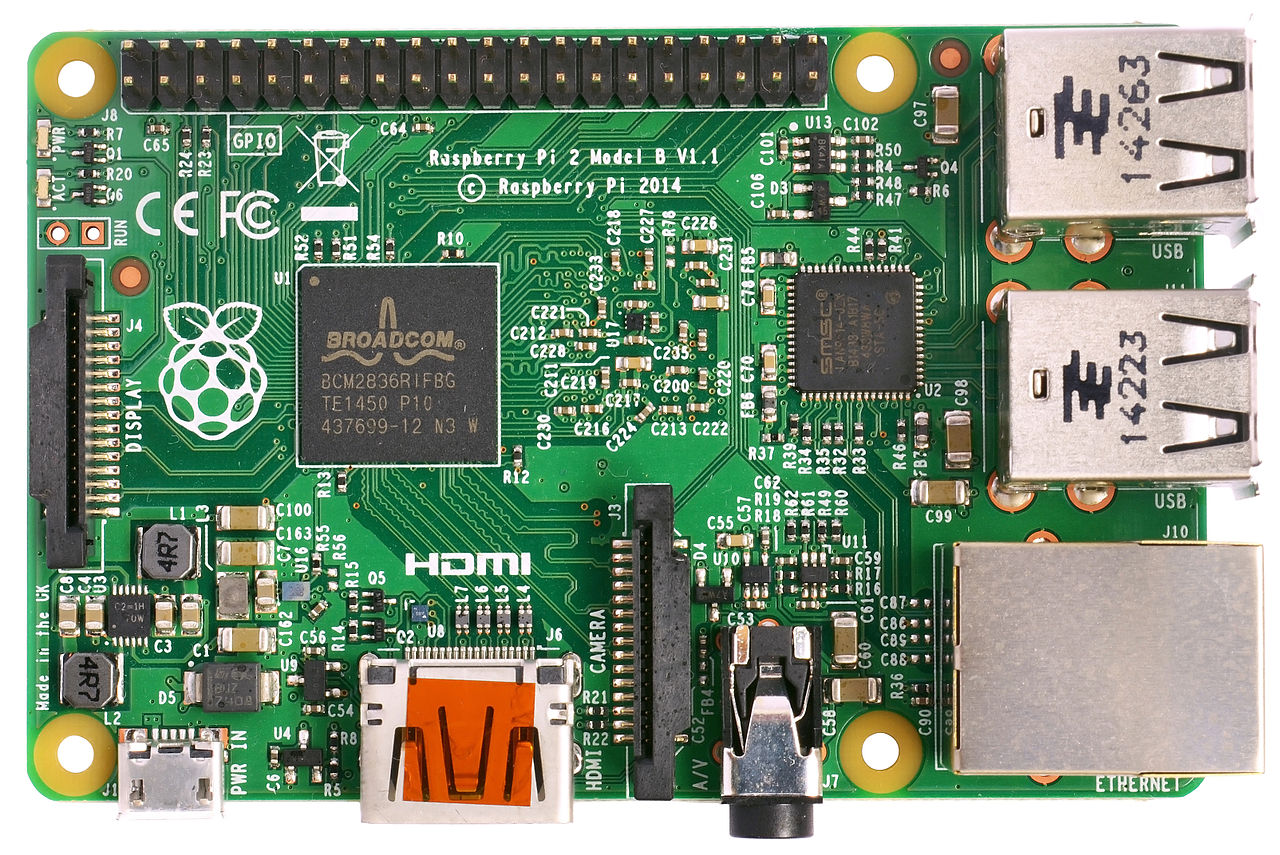
\includegraphics[width=70mm, height=40mm]{imagenes/capitulo5/5_1_RaspberryPI}
   \caption{Raspberry PI 2 model B}
   \label{5_1:Hardware}
\end{figure}

	El programa software está implementado en C ya que es un lenguaje de programación que posee características propias de los lenguajes de alto nivel y también permite manejar y gestionar la memoria y los puertos GPIO de la Raspbery PI de una forma sencilla.

	Cada bloque esta formado por un fichero \textbf{.c} y un fichero \textbf{.h}. El fichero \textbf{.c} contiene el código fuente de las funciones públicas y estáticas, así como las dependencias con otras librerías. El fichero \textbf{.h} contiene las macros y estructuras definidas, así como el prototipo de las funciones públicas implementadas en el fichero \textbf{.c}. En los siguientes apartados se detalla la implementación de cada bloque.

\section{Bloque de adquisición}\label{implementacion:adquisicion}

	La implementación de este bloque se encuentra en los ficheros \textbf{platformDown.c} y \textbf{platformDown.h}. Para facilitar dicha implementación, se han usado las librerías externas \textit{curl} \cite{curl} y \textit{jansson} \cite{jansson} para realizar las peticiones http y manejar los objetos en formato JSON respectivamente. A continuación se muestra la documentación de este modulo.

\noindent\Large\textbf{Macros definidas}\label{adquisición:macros}

\lstinputlisting[style=macros,firstline=1, lastline=10,texcl=true]{ficheros/platformDown.c}

\noindent\Large\textbf{Estructuras Definidas}\label{adquisición:estructuras}

\normalsize\textbf{struct objJSON}\label{estructuraobjJSON}
\lstinputlisting[style=estructura,firstline=15, lastline=21,texcl=true]{ficheros/platformDown.c}

\normalsize\textbf{struct temp\_leida}\label{estructuratempLeida}
\lstinputlisting[style=estructura,firstline=26, lastline=32,texcl=true]{ficheros/platformDown.c}

\noindent\Large\textbf{Funciones estáticas definidas}\label{adquisicion:functEstaticas}

\normalsize\textbf{escribir\_objeto()}\label{adquisicion:escribirObjeto}

\lstinputlisting[style=funcion,firstline=34, lastline=47,texcl=true]{ficheros/platformDown.c}

\noindent\Large\textbf{Funciones publicas definidas}\label{adquisicion:funPublicas}

\normalsize\textbf{solicitar\_objeto()}\label{adquisicion:solicitarObjeto}

\lstinputlisting[style=funcion,firstline=50, lastline=60,texcl=true]{ficheros/platformDown.c}

A conitnuación se incluye su pseudocódigo para facilitar su compresión.

\lstinputlisting[style=pseudocodigo,texcl=true]{ficheros/solicitar_objeto.c}

\normalsize\textbf{extraer\_temperatura()}\label{adquisicion:extraerTemperatura}

\lstinputlisting[style=funcion,firstline=63, lastline=72,texcl=true]{ficheros/platformDown.c}

A conitnuación se incluye su pseudocódigo para facilitar su compresión.

\lstinputlisting[style=pseudocodigo,texcl=true]{ficheros/extraer_temperatura.c}

\section{Bloque de comparación}\label{implementacion:comparacion}

	La implementación del bloque de comparación se encuentra en los ficheros \textbf{comparador.c} y \textbf{comparador.h}. Este módulo sólo dispone de la función \textit{calcular\_error()}. A continuación se incluye su documentación.

\textbf{calcular\_error()}\label{comparacion:calcularError}
\lstinputlisting[style=funcion,texcl=true]{ficheros/comparador.c}

\section{Bloque de control}\label{implementacion:control}

	La implementación de este bloque se encuentra en los ficheros \textbf{PID.c} y \textbf{PID.h}. A continuación se incluye la documentación de este módulo.

\noindent\Large\textbf{Macros definidas}\label{control:macros}

\lstinputlisting[style=macros,firstline=1, lastline=9,texcl=true]{ficheros/PID.c}

\noindent\Large\textbf{Funciones definidas}\label{control:funciones}

\normalsize\textbf{calcular\_tempcontrol()}\label{control:calcularTempControl}

\lstinputlisting[style=funcion,firstline=11, lastline=24,texcl=true]{ficheros/PID.c}

	La implementación del PID se basa en la expresión matemática del controlador PID discreto que aparece en la sección \ref{subsec:discretizacionPID}. El proceso consiste en ir calculando resultados parciales de esa fórmula y sumarlos todos para obtener el resultado final. El orden de operación es el siguiente:

\begin{enumerate}  
\addtolength{\itemsep}{-1mm}
\item Se calculan los productos y divisiones que conforman los coeficientes $q_{0}$, $q_{1}$ y $q_{2}$.
\item Se calculan los coeficientes $q_{0}$, $q_{1}$ y $q_{2}$.
\item Se calculan los productos de cada coeficiente con los valores de la señal de error.
\item Se suman los resultados de esos productos con el valor de la señal de control en el instante $n-1$, obteniendo el valor de la señal de control $m(n)$.
\end{enumerate}

	Esta función maneja números reales con una precisión de milésimas pero están expresados como números enteros. En el caso de las sumas y las restas no existen problemas de desbordamiento porque los números no son muy grandes. Sin embargo, en el caso de la multiplicación y división sí se manejan números muy grandes por lo que puede darse el caso de que al realizar este tipo de operaciones, se produzca desbordamiento u \textit{overflow} y el resultado generado sea incorrecto. Para solucionar este problema, se ha decidido implementar la multiplicación y división del siguiente modo:

\textbf{Implementación de la multiplicación}

	Supongamos 2 números reales A y B cada uno con una precisión de milésimas. A y B pueden ser expresados como la suma de su parte entera más su parte decimal.

\begin{equation*}
	\begin{aligned}
	A &= [A_{2}A_{1}A_{0},a_{1}a_{2}a_{3}] = \left( A_{2}A_{1}A_{0} + \frac{a_{1}a_{2}a_{3}}{1000}\right) \\
	B &= [B_{2}B_{1}B_{0},b_{1}b_{2}b_{3}]  = \left( B_{2}B_{1}B_{0} + \frac{b_{1}b_{2}b_{3}}{1000}\right)
	\end{aligned}
\end{equation*}

	Por tanto, el producto de A y B (A $\ast$ B) se obtiene realizando los subproductos de cada término de A por cada término de B. Dichos subproductos son:

\begin{equation*}
      \begin{aligned}
	 S_{p1} &= A_{2}A_{1}A_{0} \ast  B_{2}B_{1}B_{0} \rightarrow S_{p1} \text{(milésimas)} =  S_{p1} \ast 1000 \\
	 S_{p2} &= A_{2}A_{1}A_{0} \ast \left(\frac{b_{2}b_{1}b_{0}}{1000}\right) \rightarrow  S_{p2} \text{(milésimas)} = A_{2}A_{1}A_{0} \ast b_{2}b_{1}b_{0}\\
	 S_{p3} &= \left(\frac{a_{2}a_{1}a_{0}}{1000}\right) \ast B_{2}B_{1}B_{0} \rightarrow  S_{p3} \text{(milésimas)} = a_{2}a_{1}a_{0} \ast B_{2}B_{1}B_{0}\\
	 S_{p4} &= \left(\frac{a_{2}a_{1}a_{0}}{1000}\right) \ast \left(\frac{b_{2}b_{1}b_{0}}{1000}\right) \rightarrow  S_{p4} \text{(milésimas)}  = \left(\frac{a_{2}a_{1}a_{0} \ast b_{2}b_{1}b_{0}}{1000}\right) \\
      \end{aligned}
\end{equation*}

	Por tanto el resultado final es sumar cada uno de los subproductos expresado milésimas. De esta forma se evita el desbordamiento ya que la mayoría de los subrproductos generan el resultado directamente en milésimas sin necesidad de aplicar factores de conversión. Aquellos que no lo generan se les aplica el factor una vez se ha realizado el subproducto, lo que evita el manejo de números muy grandes. 

\noindent\textbf{Implementación de la división}

	Supongamos 2 números A y B cada uno con una precisión de milésimas. No se puede hacer la división con ambos números en las mismas unidades porque se pierde la parte decimal o sería necesario el uso de variables reales. Por tanto, es necesario multiplicar el dividiendo (en este caso A) por el factor de conversión de unidades a milésimas y dividir el resultado por el divisor (en este caso B). De este modo, el resultado obtenido es el mismo que si se hubiera hecho la división con números reales y truncado el resultado a milésimas. Además, se puede hacer la operación usando números enteros. A continuación se muestra un ejemplo de este proceso: 
\begin{equation*}
	\begin{aligned}
		A &= 13,135; \quad B = 4,328; \quad\rightarrow A/B = 3,0348 \sim 3,034 \text{ unidades} \rightarrow  3034 \text{ milésimas} \\
       		A &= 13,135 \ast 1000 ; \quad B = 4,328;    \quad\rightarrow A/B = 3034,8 \sim 3034 \text{ milésimas} 
	\end{aligned}
\end{equation*}
Hay que señalar que aunque este proceso se ha aplicado para números reales con una precisión de milésimas, es también aplicable para números reales con otra precisión aunque hay que tener en cuenta el tamaño de las variables que se estén usando.

\section{Bloque de generación de comandos}\label{sec:comandos}

	La implementación de este bloque y de los subbloques que lo componen se encuentra en los ficheros \textbf{comandos.c} y \textbf{comandos.h}. La implementación de cada subbloque se ha realizado en diferentes funciones para facilitar su modularidad. A continuación se incluye la documentación de este módulo.

\noindent\Large\textbf{Macros definidas}\label{comandos:macros}

\lstinputlisting[style=macros,firstline=1, lastline=40,texcl=true]{ficheros/comandos.c}

\noindent\Large\textbf{Estructuras definidas}\label{comandos:estructuras}

\normalsize\textbf{struct comando}\label{comandos:comando}

\lstinputlisting[style=estructura,firstline=43, lastline=49,texcl=true]{ficheros/comandos.c}

\normalsize\textbf{struct cmd\_modulado}\label{comandos:cmdModulado}

\lstinputlisting[style=estructura,firstline=51, lastline=59,texcl=true]{ficheros/comandos.c}

\noindent\Large\textbf{Funciones definidas}\label{comandos:funciones}

\normalsize Cada subbloque se ha implementado en diferentes funciones para facilitar su modularidad. A continuación se documentan las funciones de cada subbloque.

\subsection{Subbloque de selección del comando}\label{comandos:seleccion}

	La funcionalidad de este bloque se ha implementado mediante las funciones \textit{seleccionar\_setpoint()} y \textit{obtener\_comando()}. A continuación se documentan dichas funciones.

\normalsize\textbf{seleccionar\_setpoint()}\label{seleccion:setpoint}
\lstinputlisting[style=funcion,firstline=62, lastline=69,texcl=true]{ficheros/comandos.c}

\normalsize\textbf{obtener\_comando()}\label{seleccion:obtenerComando}
\lstinputlisting[style=funcion,firstline=72, lastline=81,texcl=true]{ficheros/comandos.c}

\subsection{Subbloque de modulación del comando}\label{comandos:modulacion}

Este subbloque se ha implementado con la función estática \textit{modular\_bit()} y la función \textit{modular\_comando()}. A continuación se documentan ambas funciones.

\normalsize\textbf{modular\_bit()}\label{modulacion:bit}
\lstinputlisting[style=funcion,firstline=84, lastline=96,texcl=true]{ficheros/comandos.c}

\normalsize\textbf{modular\_comando()}\label{modulacion:comando}
\lstinputlisting[style=funcion,firstline=99, lastline=110,texcl=true]{ficheros/comandos.c}

Como se ha mencionado en el apartado \ref{subsec:modulacion}, la modulación se realiza mediante la transmisión o no de una señal cuadrada de periodo $T_{carrier}$ y con una duración igual al tiempo de bit, dependiendo de sí se envía un '1'~ o un '0'. También se ha mencionado en la sección \ref{subsec:conversor} que se va a utilizar la interfaz SPI disponible en la raspberry PI para transmitir el comando al circuito emisor de infrarrojos. La modulación de cada bit se implementa del siguiente modo:

\begin{enumerate}
 \item \textbf{Modulación de un '0':} se implementa mediante una secuencia todo '0's.
 \item \textbf{Modulación de un '1':} se implementa mediante una secuencia de '1's y '0's alternados.
\end{enumerate}

	Ambas secuencias poseen la misma longitud y es el resultado de dividir el doble del periodo de bit por el periodo de la portadora (\textit{T\_carrier}). El motivo de dividir por el doble del periodo de bit es para conseguir la frecuencia deseada.

	Un factor que hay que considerar en la implementación de la modulación es que la interfaz SPI sólo permite transferencias byte a byte y que por cada byte transmitido, introduce un bit de parada. Por tanto, estos bits de parada deben ser considerados en la secuencia de modulación para que el comando modulado pueda ser interpretado por el aire acondicionado. Si no son considerados estos bits de parada, la modulación no se realiza correctamente y el aire acondicionado no podrá interpretar la orden.

	Por tanto, por cada 9 bits de la secuencia de modulación, debe ser descontado un bit de dicha secuencia, que será sustituido por el bit de parada. Este proceso se irá realizando de forma simultánea al proceso de generación del comando modulado. Sin embargo, este proceso depende de la posición de inicio de la secuencia de modulación de cada bit, ya que puede incluir más o menos bits de parada. 

\noindent Por tanto, el proceso de modulación consta de los siguientes pasos:

\begin{enumerate}
\item Se extrae de la cabecera el periodo de bit y el periodo de la portadora y se calcula la longitud de la secuencia de modulación de cada bit. 
\item Se calcula la longitud total de la secuencia de modulación del comando y los bits de parada que van a ser usado en dicha secuencia.
\item Se realiza la modulación de cada bit. Para ello, se tiene en cuenta el valor del bit, la posición de inicio de dicha secuencia dentro de una transferencia SPI, su posición final y el número de bits de parada que se van a usar en la modulación de ese bit.
\item Por último, una vez se ha realizado la modulación del comando, se comprueba que el número de bytes que ocupa dicha secuencia coincide con el número de bytes esperados y si es así devuelve un 0, indicando que la modulación se ha realizado correctamente. En caso contrario, devuelve -1.
\end{enumerate}

\section{Bloque de transmisión}\label{implementacion:transmision}

La implementación de este bloque es hardware y software. El conversor de bits a señal posee una implementación software, mientras que el circuito emisor de infrarrojos posee una implementación hardware. A continuación se detalla la implementación de ambos subbloques.

\subsection{Conversor de bits a señal}\label{sec:conversor}

La implementación de este subbloque se encuentra en los ficheros \textbf{spi.c} y \textbf{spi.h}. A continuación se incluye la documentación de este módulo.

\noindent\Large\textbf{Macros definidas}\label{conversor:macros}

\lstinputlisting[style=macros,firstline=1, lastline=13,texcl=true]{ficheros/spi.c}

\noindent\Large\textbf{Funciones definidas}\label{conversor:funciones}

\normalsize\textbf{transmitir\_comando()}

\lstinputlisting[style=funcion,firstline=16, lastline=23,texcl=true]{ficheros/spi.c}

	La función inicializa la librería pigpio y configura los puertos de la interfaz SPI. Después, crea un manejador SPI con el que realizar la transmisión y configura dicho dispositivo, incluyendo la frecuencia de bit. Por último, activa dicho dispositivo y transmite cada uno de los bytes del comando modulado. 

\subsection{Circuito emisor de infrarrojos}\label{conversor:circuito}

	Este circuito se ha implementado en una placa de inserción y se ha utilizado un diodo LED de infrarrojos LD271, un transistor BJT npn y 2 resistencias. Las características del circuito son las siguientes:\\ \\
           \textbf{Tensión de alimentación:} $V_{CC}=5V$. \\
	\textbf{Tensión y corriente del diodo:} $V_{D}=1,3V$ y $I_{D}=130mA$. \\
	\textbf{BJT en corte:} $I_{C} = I_{B} = 0$. \underline{Condición:} $V_{BE}<V_{\gamma E}$.\\ 
          \textbf{BJT en saturación:} $V_{BE} = V_{\gamma E}$, $V_{CE} = V_{CE(SAT)}$. \underline{Condiciones:} $I_{C}<\beta I_{B}$, $ I_{B}>0$.\\
           \textbf{Parámetros transistor:} $\beta=100$, $V_{CE(SAT)}=0,2V$ y $V_{\gamma E}=0,7V$. \\
           \textbf{Señal de entrada:} es una señal digital de valores $V_{HIGH}=3,3V$ y $V_{LOW}=0V$.

A continuación se muestra el análisis del circuito suponiendo que el transistor está en saturación. No es necesario hacerlo en corte porque en ese estado no circula corriente por el circuito y se alcanzaría dicho estado con cualquier valor de R1 y R2.
\begin{gather*} 
V_{R2} = V_{CC} - V_{D} - V_{CE(SAT)} = 5 - 1,3 - 0,2 = 3,5 V \\
\boxed{R2 = \frac{V_{R2}}{I_{D}} = 26,92 \Omega }\\ 
I_{B} > \frac{I_{C}}{\beta} = 1,3 mA  \quad \text{Se elige} \quad  I_{B}=16 mA\\
\boxed{R_{1}= \frac{V_{IN}-V_{BE(SAT)}}{I_{B}}=\frac{3,3-0,7}{0,016}=162,5 \Omega}
\end{gather*}
Por tanto, los valores de los componentes son: \fbox{$R_{1}=160\Omega \pm 5\%$  y $R_{2} = 27\Omega \pm 5\%$}

Por último, en la figura \ref{circuitoIR} se muestra el circuito de infrarrojos implementado. Hay que indicar que la resistencia $R_{1}$ se ha hecho conectando varias resistencias en serie que equivalen a su valor. 

\begin{figure}[htbp]
	\centering
	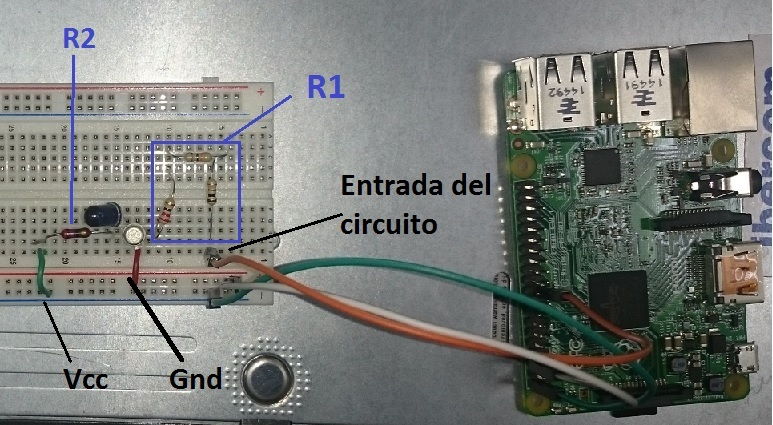
\includegraphics[width=115mm, height=50mm]{imagenes/capitulo5/circuitoIR}
   	\caption{Imagen del circuito de infrarrojos}
   	\label{circuitoIR}
\end{figure}

\section{Bloque de envío de datos}\label{implementacion:envioDatos}

La implementación de este bloque se encuentra en los ficheros \textbf{platformUp.c} y \textbf{platformUp.h}. Este módulo sólo contiene la función \textit{enviar\_datos()}. A continuación se incluye su documentación.

\lstinputlisting[style=funcion,texcl=true]{ficheros/platformUp.c}

\section{Ciclo de ejecución}\label{implemnetacion:actuador}

La implementación del ciclo de ejecución está en el fichero \textbf{actuador.c}. En este fichero se encuentra la función \textit{main()} que se encarga de realizar el ciclo del actuador y coordinar cada una de las etapas. A continuación se muestra el pseudocógido de dicha función.

\lstinputlisting[style=pseudocodigo,texcl=true]{ficheros/actuador.c}


